\documentclass[letterpaper, 12 pt, conference]{IEEEtran}  
\IEEEoverridecommandlockouts                              
%\overrideIEEEmargins
\usepackage[utf8]{inputenc}
\usepackage[T1]{fontenc}
\usepackage{hyperref}
\usepackage{xcolor}
\usepackage{graphicx}
\usepackage{amsmath}
\graphicspath{{./images/}} 


\title{Non-deterministic Search and Simulated Annealing}
% author names and affiliations
\author{\IEEEauthorblockN{Siddhesh Bhosale}
\IEEEauthorblockA{202051177}
\IEEEauthorblockA{}
\and
\IEEEauthorblockN{Rishi Raj Sachan}
\IEEEauthorblockA{202051158}
\and
\IEEEauthorblockN{Shreyansh Chachaundiya}
\IEEEauthorblockA{202051175}
\and
\IEEEauthorblockN{Nitin Kumar Das}
\IEEEauthorblockA{202051128}
}

\begin{document}
\maketitle
%\thispagestyle{empty}
%\pagestyle{empty}

\setlength{\parindent}{20pt}
\begin{center}
Course Instructor: Dr. Pratik Shah
\end{center}
\begin{center}
Group Name : AI Elites
\end{center}
\begin{center}
\noindent Github link: \href{https://github.com/ShreyanshChachaundiya/AI_LABS/tree/main/Lab3}{LAB-8}
\end{center}
\maketitle

\section{Introduction}
MENACE is a machine that learns how to play noughts and crosses through repetitive gameplay against an opponent. Over time, it improves its strategy until it reaches a near-perfect level, allowing it to either win or draw every game. This process is comparable to the way a neural network begins with random optimization before refining its performance. The learning method utilized is called Reinforcement Learning, where the machine is rewarded for drawing or winning, but punished for losing. Each matchbox in the machine represents a specific layout of the noughts and crosses board, but instead of requiring a matchbox for every unique layout, rotated versions or symmetrical layouts are grouped together to reduce the necessary number of boxes to 304.
\section{Training MENACE}
At the start, each matchbox in MENACE contains beads of different colors that correspond to moves or positions on the noughts and crosses board. Similar to a neural network's weights, these beads represent the current state of the game. When it's MENACE's turn to make a move, a human player randomly selects a bead from the relevant matchbox, which determines where MENACE will play based on the color of the selected bead.
\section{ Cumulative Reward Equation}
Let B1(i) be the number of beads of color I in the first matchbox, where I ranges from 1 to N, the total number of colors.\\\\
After each game, the number of beads in the first box is adjusted according to the following rules:\\\\
If MENACE loses, then B1(i) = B1(i) - Mi(i), where Mi(i) is the number of beads of color I used by MENACE in the game.\\\\
If MENACE wins, then B1(i) = B1(i) + 3Wi(i), where Wi(i) is the number of beads of color I used by MENACE in the game.\\\\
If the game results in a draw, then B1(i) = B1(i) + Di(i), where Di(i) is 1 if MENACE used color I during the game, and 0 otherwise.\\\\
After many games are played out, the matchboxes will have
more of some beads than the others. This certainly tinkers
with the probability of a bead being selected randomly which
changes the probability of the next state after every move.\\

\section{Analysis  Results}

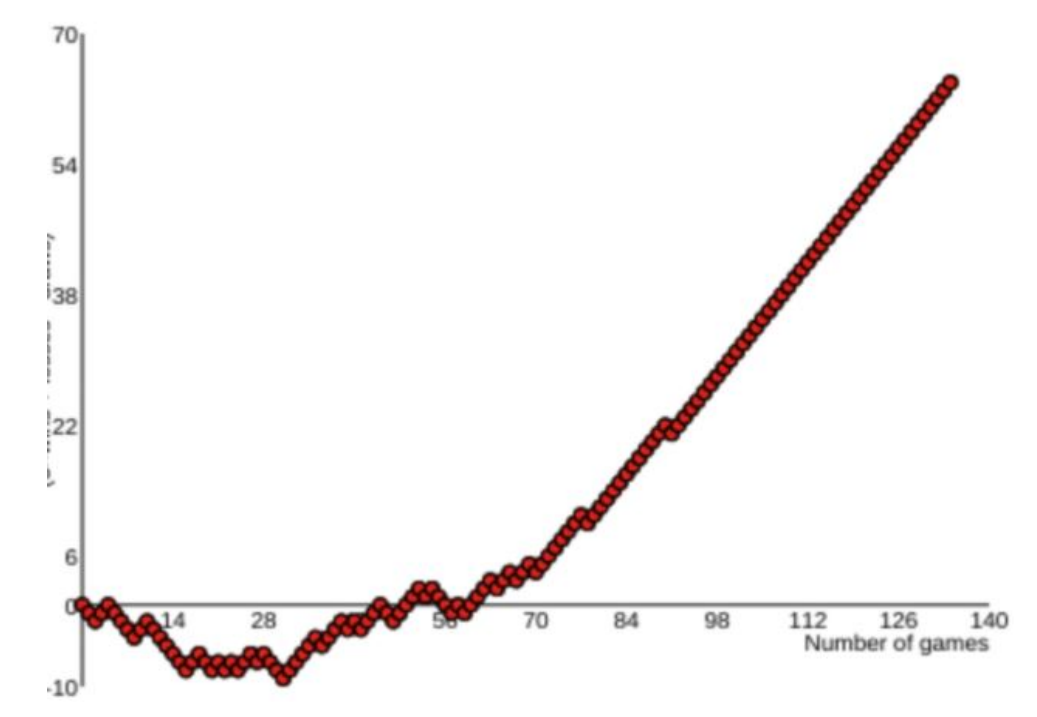
\includegraphics[width=9cm, height=5cm]{1.png}
Figure: Variation of Reward Equation (Y axis) with number\\\\
The graph demonstrates that when MENACE played against a computer with a perfect playing strategy, the value of the equation initially decreased, indicating that MENACE suffered losses. However, the value gradually increased over time, indicating that MENACE learned and improved its performance. Although the number of wins increased only slightly, draws were considered positive outcomes, leading to a positive trend in the equation value. The graph suggests that MENACE was unable to achieve victory against the perfect algorithm, but after approximately 90 games, it consistently achieved a draw, making it equally as skilled as the computer.
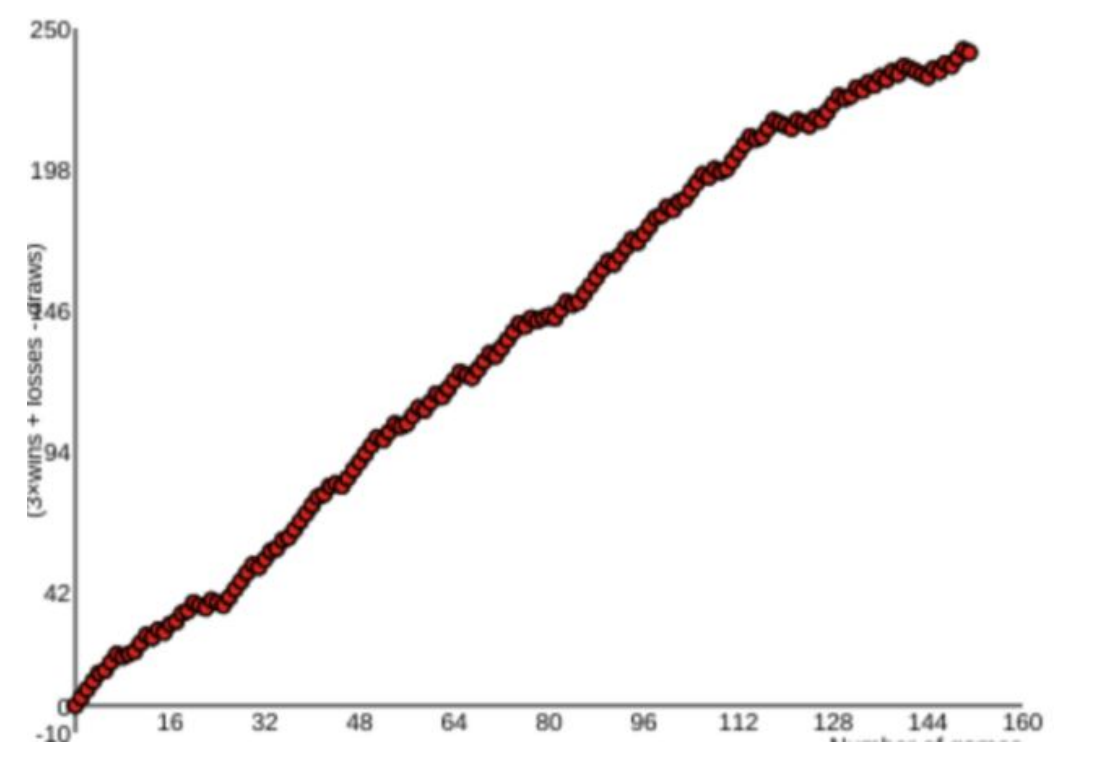
\includegraphics[width=9cm, height=5cm]{2.png}
Figure: Variation of Reward Equation (Y axis) with number
of games (X axis) for Menace against Unintelligent
Machine\\\\
In contrast, when MENACE played against an opponent who made random moves, the result showed a near-perfect positive correlation. This suggests that MENACE had a very low tendency to lose against an unintelligent player, even though MENACE also made random moves in the beginning. The equation value never became negative, indicating that MENACE's performance was consistently better than that of the random opponent.

\end{document}
